\documentclass[a4paper,10pt,twoside]{article}
\usepackage{its_conf}
\begin{document}
\setcounter{section}{0}
\setcounter{figure}{0}
\setcounter{table}{0}
\setcounter{equation}{0}
\setcounter{secnumdepth}{1}
\setcounter{secnumdepth}{1}





% =================================================================== Lab report 2 =============================================================================





\topic{Schlierin imaging techniques for visualising shock boundary layer interactions}





\information{S. D. Tomlinson - Lab report 2}
{CID - 01255194}
{Department of Aeronautics, Imperial College London SW7 2AZ}
{sdt@ic.ac.uk}





% ==================================================================== Abstract ===============================================================================





\annotation{In this report a method of extraction of information about a governing flow field is presented using Schlierin imaging. The complex interaction between a shock wave and boundary is introduced, which occur in a large range of supersonic flows. This method is outlined, flow set-up and experimental procedure and this is the interaction observed using image processing techniques with different methods are used. Vertical and horizontal knife edge measurement at a low sampling frequency allow for limited analysis of frequencies but allow for the determination that the reflected shock is unsteadier. Then vertical high frequency images allow for the deduction of oscillatory frequency of our system for all incident, reflected wave and shock bubble. This the allows for a comparative evaluation of the Strouhal number and thus the conclusion that the flow dynamics are due to a down not upstream mechanism. Lastly some ideas for future development are given. }






\begin{multicols}{2} 





% ================================================================== Introduction ==============================================================================





\section{Introduction}





In light of first imagining how to visualise waves in compressible gases, one may ask, how is it possible to see the invisible? Schlierin imaging techniques are one of many interferometric techniques used to answer this question, which exploit and analyse density changes in a moving fluid \cite{1}. It was first known to be practiced by physicist Robert Hooke, who used an elementary set-up of lens and eye, in the attempt of visualising thermal plumes from a candle \cite{1}. Its general principles are maybe best explained via a simple example using a cigarette lighter in the presence of a light source. Holding the lighter up so that the shadow of your hand appears on the ground and in-turn turning on this lighter, results in a bumpy turbulent shadow forming above the source. What causes this is density changes in the air which in-turn causes light to bend. This forms a shadow where this light once would of hit the ground, and a good amount of information can be gathered about the underlying flow mechanism by observing this shadow. \par



It is common knowledge that light can be treated as a wave which has a amplitude, wavelength and polarisation. Other important properties are that waves refract, meaning that the are deflected by certain changes in the field (e.g. a change of medium), they diffract meaning we have distortion, and that light waves can be dispersed [Reference]. The production of a shadow graph, which Schlierin involves, depends on changes in refraction in our medium, in which these electromagnetic waves are propagating. This process of diffraction is governed by the following equation
\begin{equation}
    n = \frac{c_0}{c},
\end{equation}
where $c_0$ and $c$ are the speeds of light, in a vacuum and in our medium. Changes in $n$ cause refraction and the displacement of these waves which in turn creates the shadow graph. Density is related to this index of refraction, $n$, by the Gladstone-Dale relation \cite{2}, which for gases is 
\begin{equation}
    n -1 = \kappa \rho,
\end{equation}
which is valid if and only if $n \approx 1$, which in our case, at essentially standard temperature and pressure, is sufficient. The Gladstone-Dale constant, $\kappa$, is also a function of these variables as well as the incident wavelength of light. For demonstrative purposed if we consider an example of a small change in density between two points in time then we have $\kappa(t_1) \approx 0.2230$ for $\rho(t_1)$ and $\kappa \approx 0.2330$ for $\rho(t_2)$, so that light rays will deflect towards regions of higher density.  \par 



\begin{figure}[H]
    \centering
    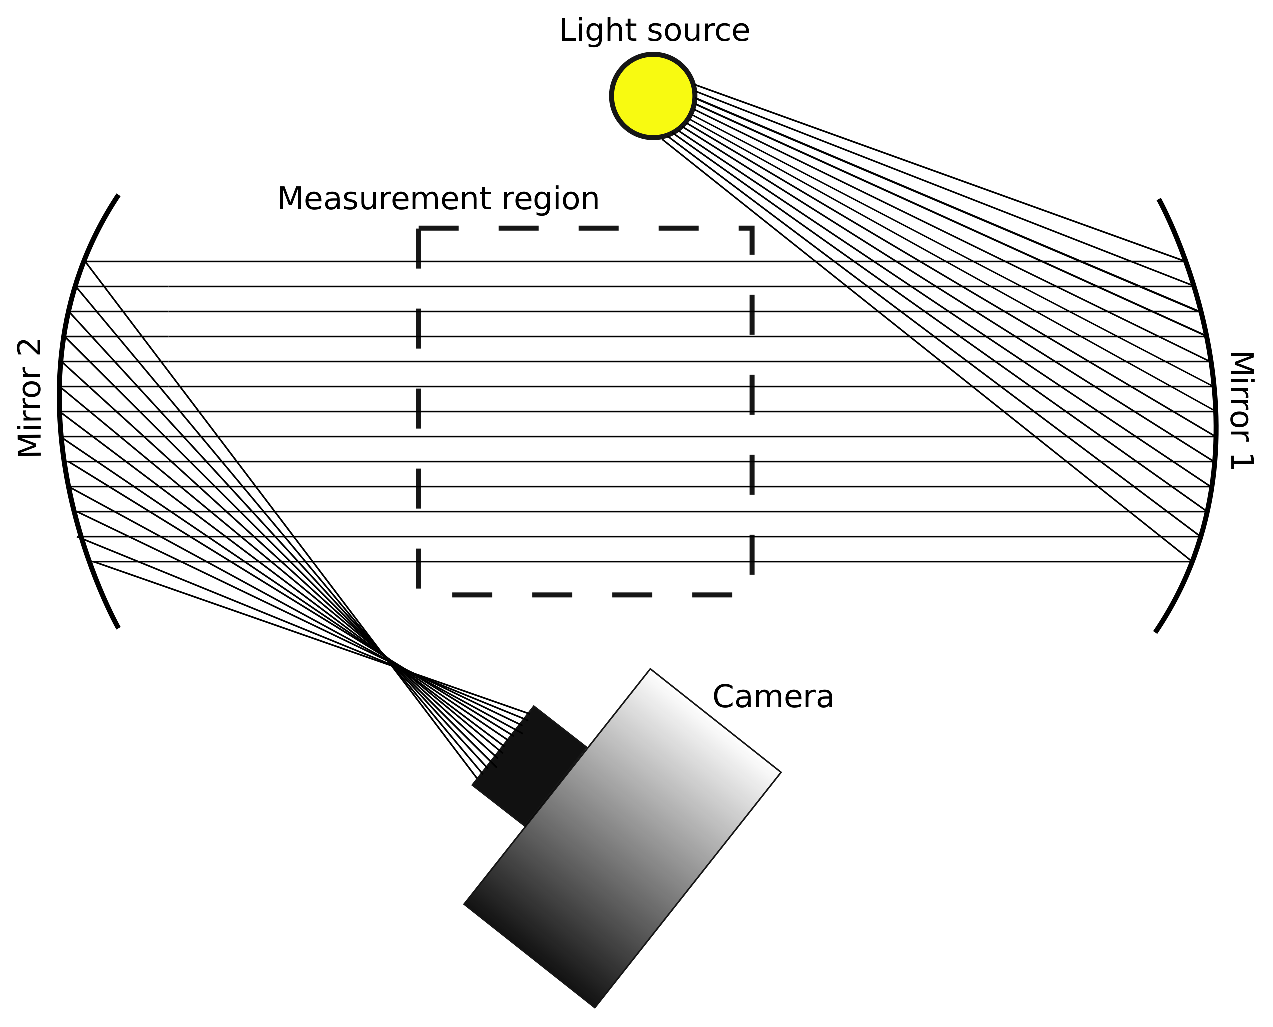
\includegraphics[width=\linewidth]{SI.eps}
    \caption{Shadow graph imaging set-up.}
    \label{fig:my_label}
\end{figure}




In our current context, that is to view shock boundary layer interactions in the test section of a supersonic wind tunnel the set up for Schlierin imaging is as follows (see Figure 1). Two lenses are used, the first collimates the light source (making the light rays more parallel). Then the light is allowed to continue in its path, through the measurement region, until it meets another lens which then focuses the light rays into a camera. The shadow graph technique is then turned into a Schlierin image by placing a spatial filter where these light beams theoretically cross (just in-front of the camera. There are many types of filters that can be used at this stage, low-pass, high-pass but the two we are interested in are heavy side filters (knife edge) which remove high and low frequency content. These filters result in the back round being uniformly dimmed and the density gradient thereby appears lighter or darker, depending on the direction in which this filter is place. [REFERENCE THIS ENTIRE PARAGRAPH]



\vspace{5mm}
\centerline{\textbf{Shock waves and boundary layers}}
\vspace{5mm}



\begin{figure}[H]
    \centering
    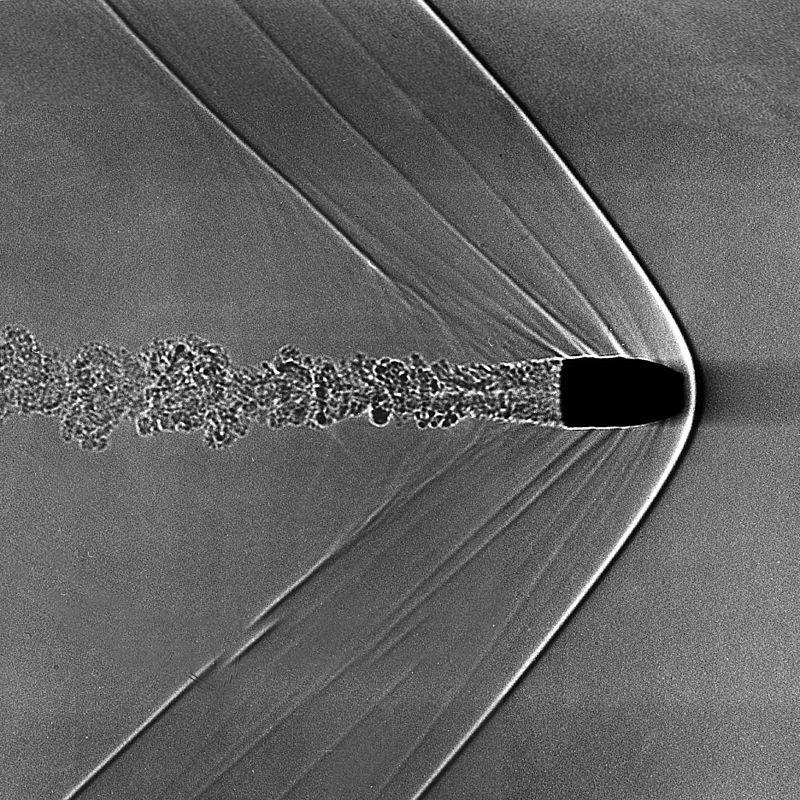
\includegraphics[width=\linewidth]{bulletshock.jpg}
    \caption{Bullet with shock waves to either side \cite{4}.}
    \label{fig:my_label}
\end{figure}



A shock wave is defined to be a propagating discontinuity across a narrow region of a medium caused in our case by the relative movement of a body faster than the speed of sound. In our particular flow set-up we have an oblique shock \cite{8} which is defined where we have an angle in which the shock is formed with the incoming free-stream as opposed to the classical example of normal shock waves. This tilt is caused by the placement of a corner in the incoming stream, which in our case is a wedge. Oblique shock-waves for a perfect gas have the following property ratios across an oblique shock \cite{8};
\begin{equation}
    \frac{\rho_2}{\rho_1} = \frac{(\gamma + 1)Ma_{n1}^2}{2+(\gamma-1)Ma_{n1}^2},
\end{equation}
\begin{equation}
    \frac{p_2}{p_1} = \frac{1}{\gamma+1}(2\gamma Ma_{n1}^2 - (\gamma-1)),
\end{equation}
\begin{equation}
    \frac{h_2}{h_1} = \frac{p_2 \rho_1}{p_1 \rho_2},
\end{equation}
and
\begin{equation}
    \frac{p_{o2}}{p_{o1}} = \frac{p_2}{p_1}\bigg(\frac{h_2}{h_1}\bigg)^{\frac{\gamma}{\gamma-1}},
\end{equation}
where $\rho_i$, $p_i$, $h_i$ ($i \in \{1,2\}$) are the density, pressure and enthalpy before/after the shock. The normal Mach numbers are defined as follows
\begin{equation}
    Ma_{n1} = Ma_1 \sin(\beta)
\end{equation}
and
\begin{equation}
    Ma_{n2} = Ma_2 \sin(\beta-\theta).
\end{equation}
Using the above equations we can arrive at an equation relating the shock angle, $\beta$, angle of the wedge and the Mach number (see appendix 1), which we will use in Section IV to calculate this angle,
\begin{equation}
    \tan(\theta) = \frac{2 \text{cot}(\beta)(Ma_{n1}^2 \sin^2(\beta) - 1) }{Ma_{n1}^2(\gamma+\cos(2\beta))+2}.
\end{equation}. 
A boundary layer is a small region where viscous effects dominate near a moving body. In our case this boundary layer is turbulent so as opposed to the standard laminar boundary layer, where fluid layers essentially slide over one another, in the supersonic flow this motion becomes sporadic and highly unpredictable. It is the interaction between these two flow phenomenon that we are interested in this report.



In the working section of this wind-tunnel, at which we will employ Schlierin imaging a certain flow configuration will ensue. This will be an incident oblique shock wave propagating at on angle $beta$ towards a wall, where some complex interaction will happen between this shock wave and the turbulent boundary layer. This shock boundary layer interaction has been a subject of a large amount of work over the last century \cite{3}, \cite{5}, \cite{6} and \cite{7}. A object called a separation bubble will form in this region of complex interaction, caused by the interaction of the incident shock wave and the separation of the boundary layer, it is debated whether the oscillations in the system are due to upstream turbulent boundary wave effects or due to the shock bubble and this postulate will be the topic of this report. \par



In this report an experimental procedure will be described, as to measure properties of these three main features of the given flow field. Schlierin imaging techniques will be employed as well as some required image processing techniques as to filter out the large amount of noise in the given flow. The low frequency oscillations of the incident wave, reflected wave and separation bubble will be evaluated as well as other properties such as the the boundary layer thickness, the shock angle, with Mach and Reynolds numbers. This will allow for comparison with previous works in which the estimated Strouhal number will be evaluated and provide insight into the governing flow mechanism.





% =============================================================== Experimental setup ===========================================================================





\end{multicols}



\begin{figure}[H]
    \centering
    \includegraphics[width=\linewidth]{Windtunnel_scematic.eps}
    \caption{Wind tunnel schematic depicting its differing sections.}
    \label{fig:my_label}
\end{figure}



\begin{multicols}{2}



\section{Experimental setup}



In Figure 3 we see a schematic of a supersonic wind tunnel. Air is taken into the chamber where it is contain and held at extremely high pressures. When it is released it enters the stagnation chamber where the increase in volume then causes this currently subsonic flow to accelerate to supersonic flow. As the stagnation then restricts this then causes further acceleration to the supersonic flow where it enters the test section and flows past our wedge. The air then enters the diffusing stage, through supersonic to subsonic basically where the flow is decelerating all the way up the column where it is released back into the air. \par 



\begin{figure}[H]
    \centering
    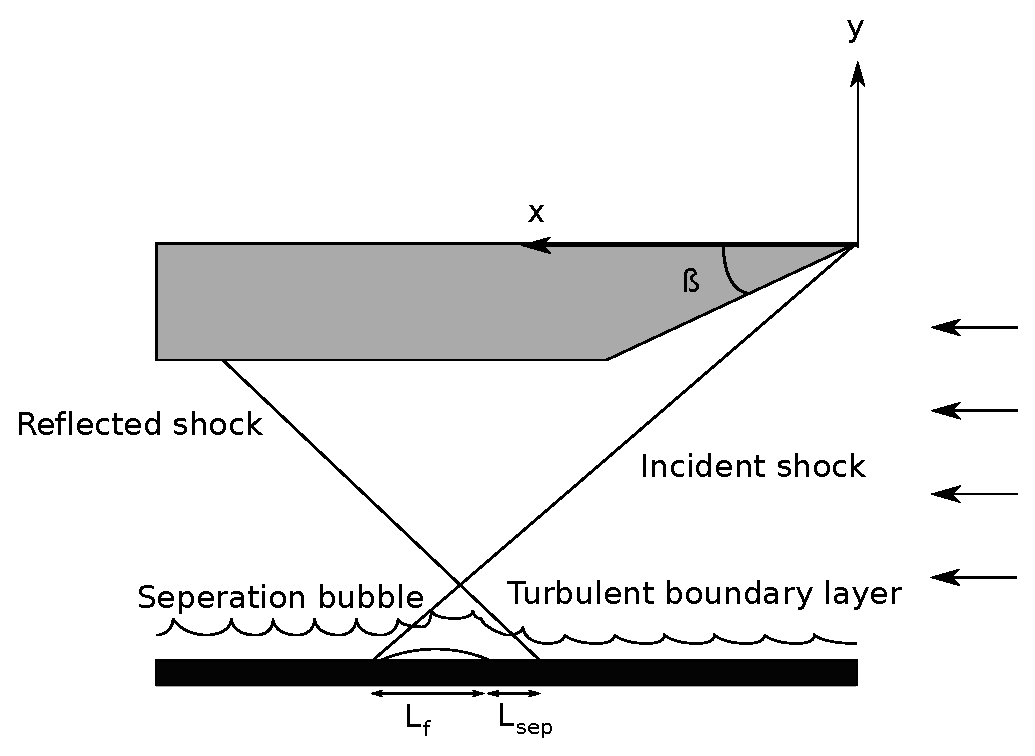
\includegraphics[width=\linewidth]{wedgeschem.eps}
    \caption{Wedge schematic depicting flow configuration with coordinate axis.}
    \label{fig:my_label}
\end{figure}



In the configuration of the wind tunnel a free stream Mach number of
\begin{equation}
    Ma = 2.0,
\end{equation}
was the desired, for which we give a better estimate in Section IV using the Shock angle, and a 10$^{\circ}$ ramp is mounted to the roof of the tunnel. \par 



The schematic of the full tunnel is given in Figure 3 but more specifically we can refer to Figure 4 and define a coordinate frame in the test section such that the start of the wedge is the origin and the stream wise ($x$-component) of velocity is defined to be $u$, the height wise ($y$-component) of velocity is defined to be $v$ and lastly the width ($z$-component) $w$. A couple of important features of the flow field are depicted here. The length scale called the separation length scale $F_{sep}$, and $L_i$, the intermediate length scale also depicted are the pre-separation and post-separation boundary layer thicknesses. We will be able to evaluate these properties in Section IV allowing for estimated Strouhal numbers using these two length scales allowing for an evaluation of the underlying mechanism. \par 





% ======================================================================== Method ===============================================================================





\section{Method}





A brief overview of the experimental procedure is given as follows;



\begin{itemize}



    \item The air tanks are filled prior to this procedure and the first stage is to record the temperature and pressure inside the wind tunnel and also (was done in some other places too).
    
    
    
    \item The classical Schlierin set-up is created (refer back to Figure 1) with two lenses redirecting light from a light source which passes over a knife edge into the camera. This is calibrated using a test of a thermal plume as close to the wind tunnel as possible. This is visualised using PCC software in live mode.
    
    
    
    \item Image sizes and frame rate settings are fixed, for the first vertical knife edge, horizontal knife edge and reduced resolution knife edge the frame rates used were 1000fps for both higher resolution and 16000fps for reduced resolution. We used resolutions of 2560x1600 for the first two and 512x384 for the lastter.
    
    
    
    \item Next the timing is synced so that initially before the wind tunnel starts a capture button is pressed as to ready the camera then when the desired flow phenomenon is observed a trigger is used to capture the image.
    
    
    
    \item The images are captured converted from a .cine to a .tiff file ready for post processing in MATLAB.
    
    
    
    \item LABVIEW \cite{9}, is used to control the tunnel via a pressure tapping before the converging-diverging nozzle. It is important to maintain a constant total pressure here and this is achieved via a PID feedback system varying air flow and the position of the control valve.
    
    
    
\end{itemize}





% ================================================================ Results and discussion =======================================================================





\section{Results and discussion}



In this section we outline the results from the experimental procedure described in the Section IV and use some image processing techniques to identify some features of the flow field, namely important frequencies such as the shock wave oscillations, for both the upstream and downstream, the turbulent boundary layer thickness and lastly some properties of the separation bubble. Before we start it is instructive to get a feel for what is going on in each of the cases for vertical and horizontal measurement and identify the measurement regions in the flow. \par



In Figure 5 we have the standard vertical knife edge image selected at random from the sample. 5 key areas are highlighted in this image. The first is the mach line which is a pressure wave which is a weak counterpart of our shock wave. We have the incident shock and reflected shock from the boundary with the region near the boundary being the shock bubble. Also in the image are some weaker wave which will play no part in this report. \par



\begin{figure}[H]
    \centering
    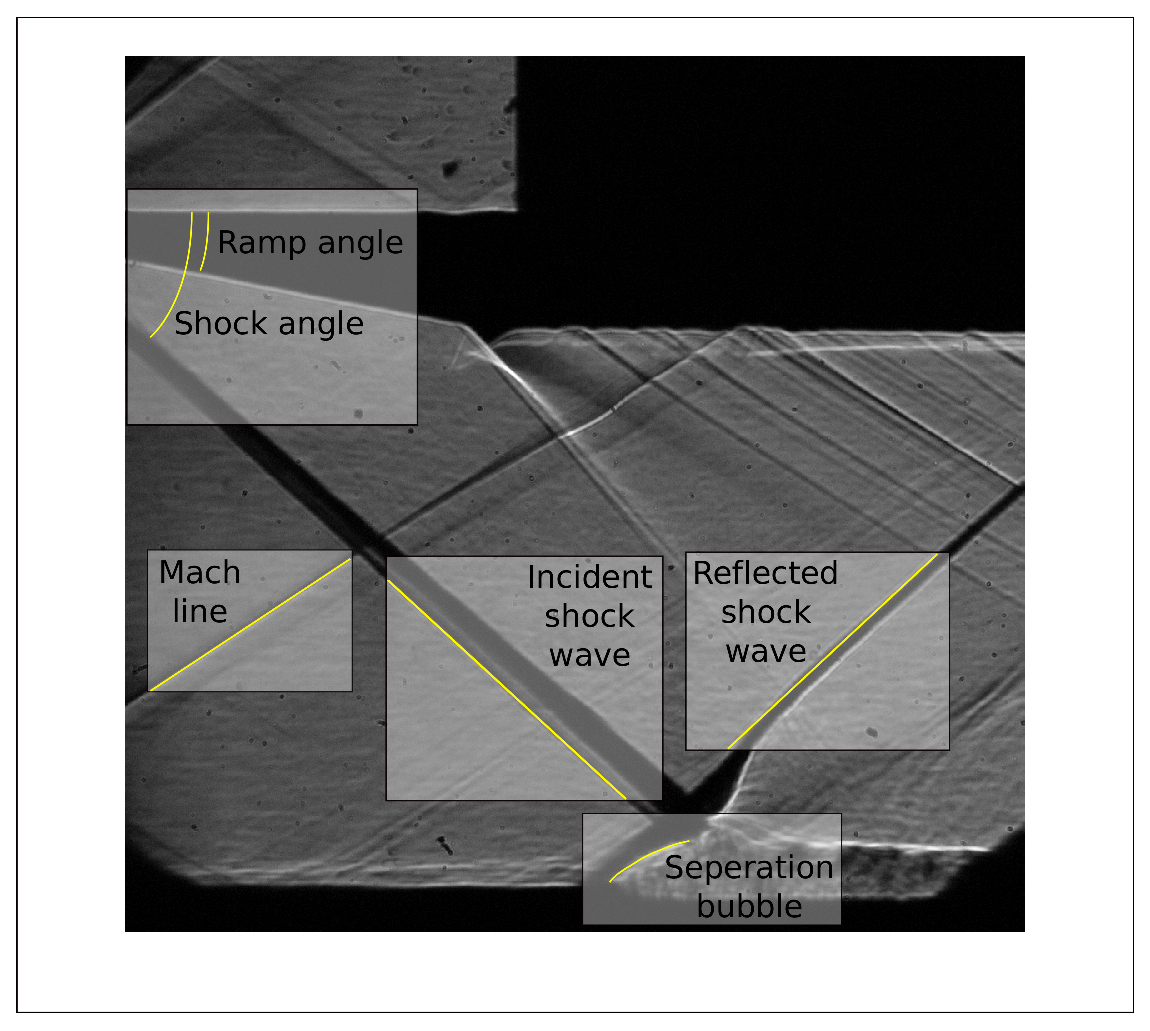
\includegraphics[width=\linewidth]{vert_highres2.eps}
    \caption{Vertical knife edge image depicting incident and reflected shock waves, mach line, separation bubble, wedge and shock angles.}
    \label{fig:my_label}
\end{figure}



Next in the horizontal image we observe a different features highlighted slightly clearer in the flow, namely the expansion fan and pre-/post-boundary layer. The reason for this difference in features is outlined in Section 1. \par



\begin{figure}[H]
    \centering
    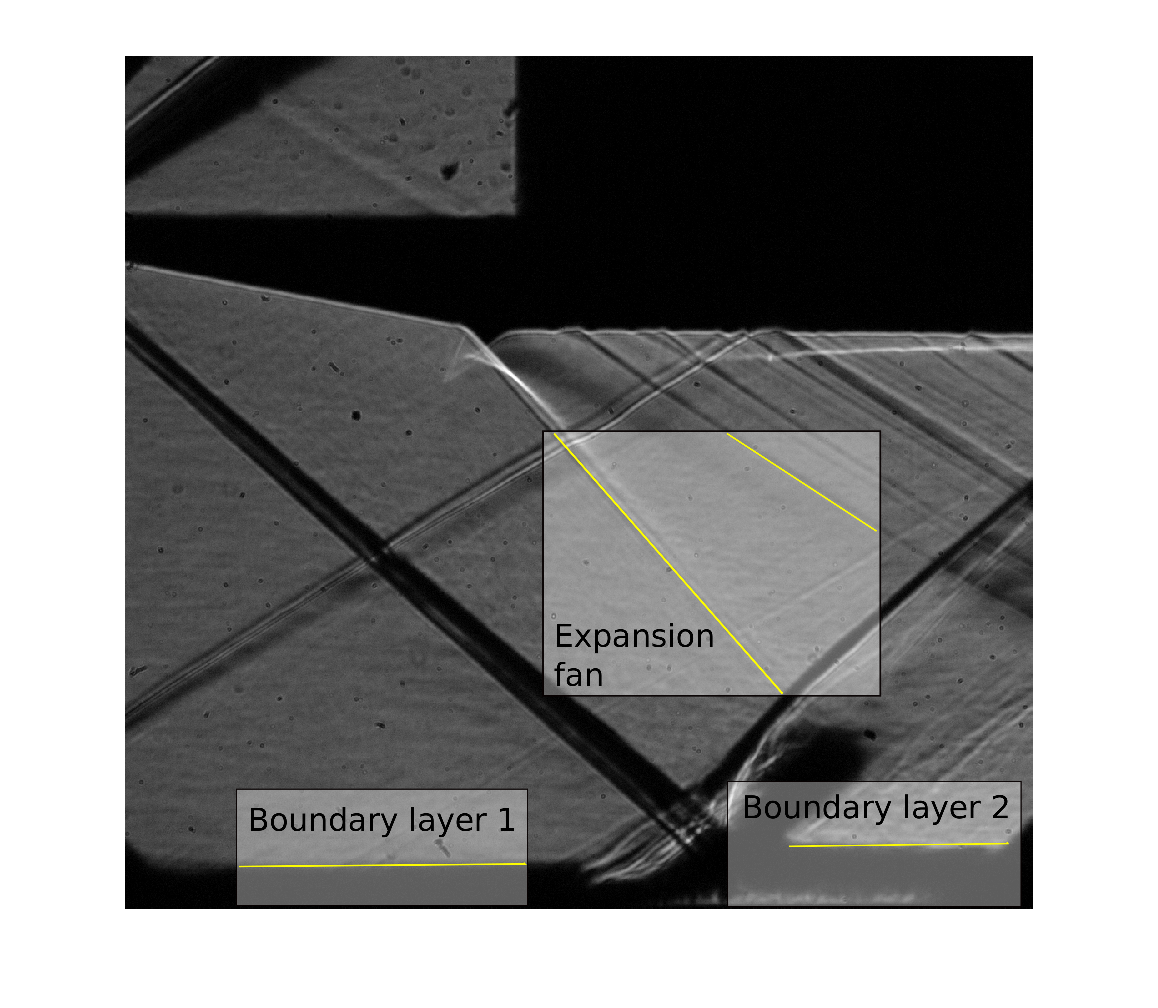
\includegraphics[width=\linewidth]{hor_highres.eps}
    \caption{Horizontal knife edge image depicting both boundary layers of differing heights and the expansion fan.}
    \label{fig:my_label}
\end{figure}



Now we will move on to analysing each of these sets of images, firstly vertical and horizontal at high resolution low sampling rate then moving on to the lower resolution high sampling to hope to capture the dynamics of the system. \par





\vspace{5mm}
\centerline{\textbf{Vertical knife edge - high resolution}}
\vspace{5mm}





In reference to Figure 2 we first go about analysing the angles of the incident and reflected shock wave and lastly the Mach line. Using various image processing techniques in which the image is filtered, edges are highlighted and then gradient of the edges are calculated. Using this and the position of the wall this allows us to work out the Shock angles, given in the following table
\begin{table}[H]
\begin{center}
\begin{tabular}{ |c|c| } 
 \hline
 Wave & Angle (4 d.p) \\
 \hline
 Incident shock wave &  $\beta_{inc} = 35.8593$ \\ 
 Reflected shock wave & $\beta_{ref} = 138.1211$ \\ 
 Mach line &  $\beta_{mach} = 146.3099$ \\
\hline
\end{tabular}
\end{center}
\caption{Table of estimated wave angles, for incdent and reflected shock waves and mach line.}
\end{table} \par



Then in reference to Section I we can use Equation (12) deverived for the equations on a oblique shock wave to get a better estimate of the free stream Mach number (4 d.p), as opposed to our aforementioned pre-set $Ma_{setup}=2.0$ to be 
\begin{equation}
    Ma = 1.8724.
\end{equation}
Using this then allows us to estimate the free-stream velocity, using the speed of sound, we have the formula
\begin{equation}
    Ma = \frac{U_{\infty}}{a},
\end{equation}
with $a=343.2m/s$, allowing us to calculate  
\begin{equation}
    U_{\infty} = 642.6077.
\end{equation}
Now taking the length scale to be that at the end of the wedge we estimate the Reynolds number of the flow to be 
\begin{equation}
    Re=\frac{U*L}{\nu} = 2124400
\end{equation} \par



Next we can evaluate the steadiness of this Shock by how it oscillates. Again tracking the position of the middle, up and bottom edge then calculating their distances in normal horizontal and vertical directions, over time. Unfortunately with all power spectrum being similarly noisy and without much to conclude from this we can evaluate the power spectrum for the incident and reflected shock waves distance in the normal direction
\begin{figure}[H]
    \centering
    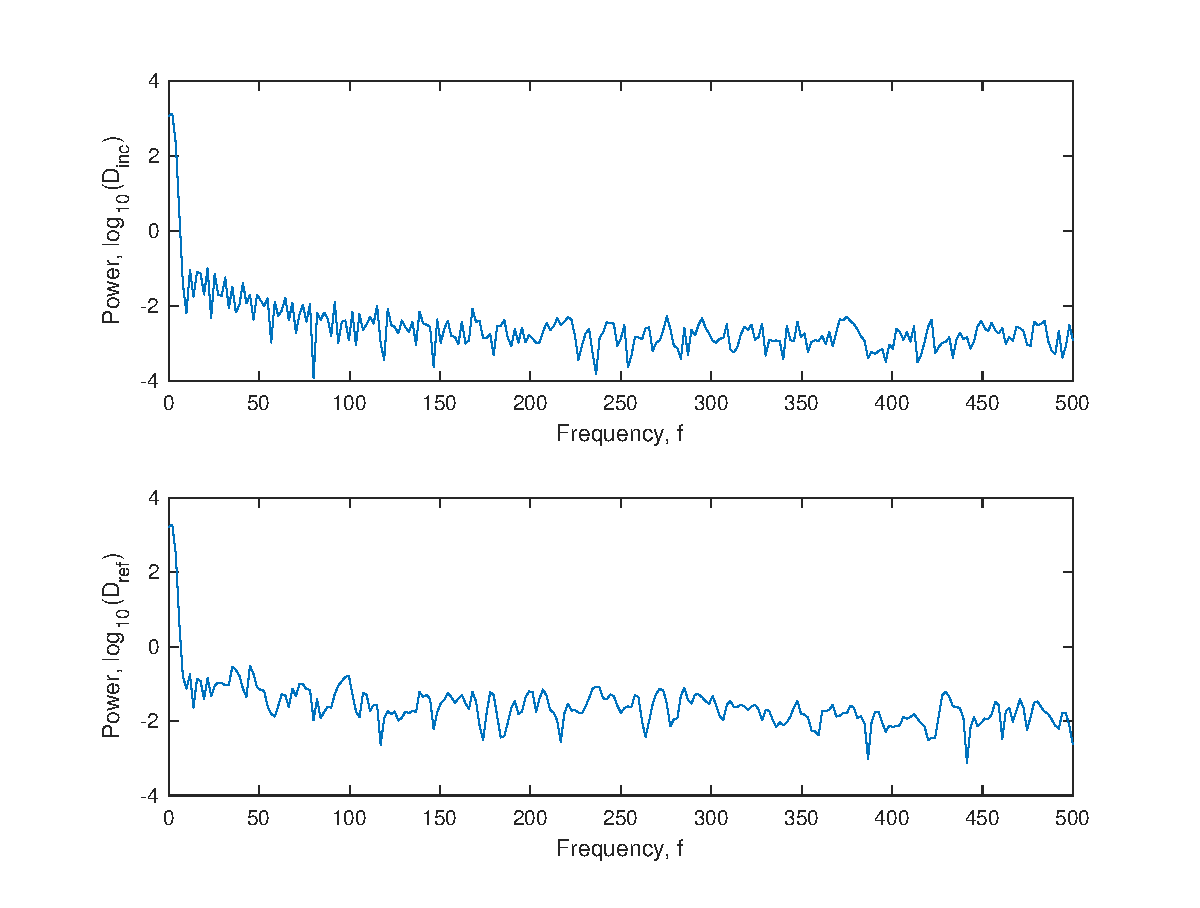
\includegraphics[width=\linewidth]{verhighres.eps}
    \caption{Power spectrum for the distance of the incident and reflected shock wave from the wall.}
    \label{fig:my_label}
\end{figure} \par


From these power spectrum there is not a massive difference visually in steadiness between the two shocks, one would be hesitant in saying that the wider breadth of frequencies in the reflected shock indicate it is more unsteady but this is by no means certain. This then prompts us the find a way by which to evaluate this unsteadiness. The larger variances in the distance data lies inside the reflected wave, the are evaluated to vertical, horizontal and normal movement, indicating that it is indeed the less steady of the two waves. This is most likely due to the separation bubbles interference having more of a prominent effect down stream, this effect would not be so large if up steam effects induced vibrations as both wave would be effected and the difference in steadiness less noticeable. \par





\vspace{5mm}
\centerline{\textbf{Horizontal knife edge - high resolution}}
\vspace{5mm}





We are now required to carry out the same analysis for the horizontal knife edge for the incident and reflected shock. One can again calculate angles, Mach and Reynolds number which have small order differences and are thereby negligible. Also the unsteadiness can be calculated and the same result observed. We immediately expect there to be more noise as this filter does not highlight the shock features of the flow as the vertical knife edge does. Indeed our spectra again for incident and reflected waves are given below.



\begin{figure}[H]
    \centering
    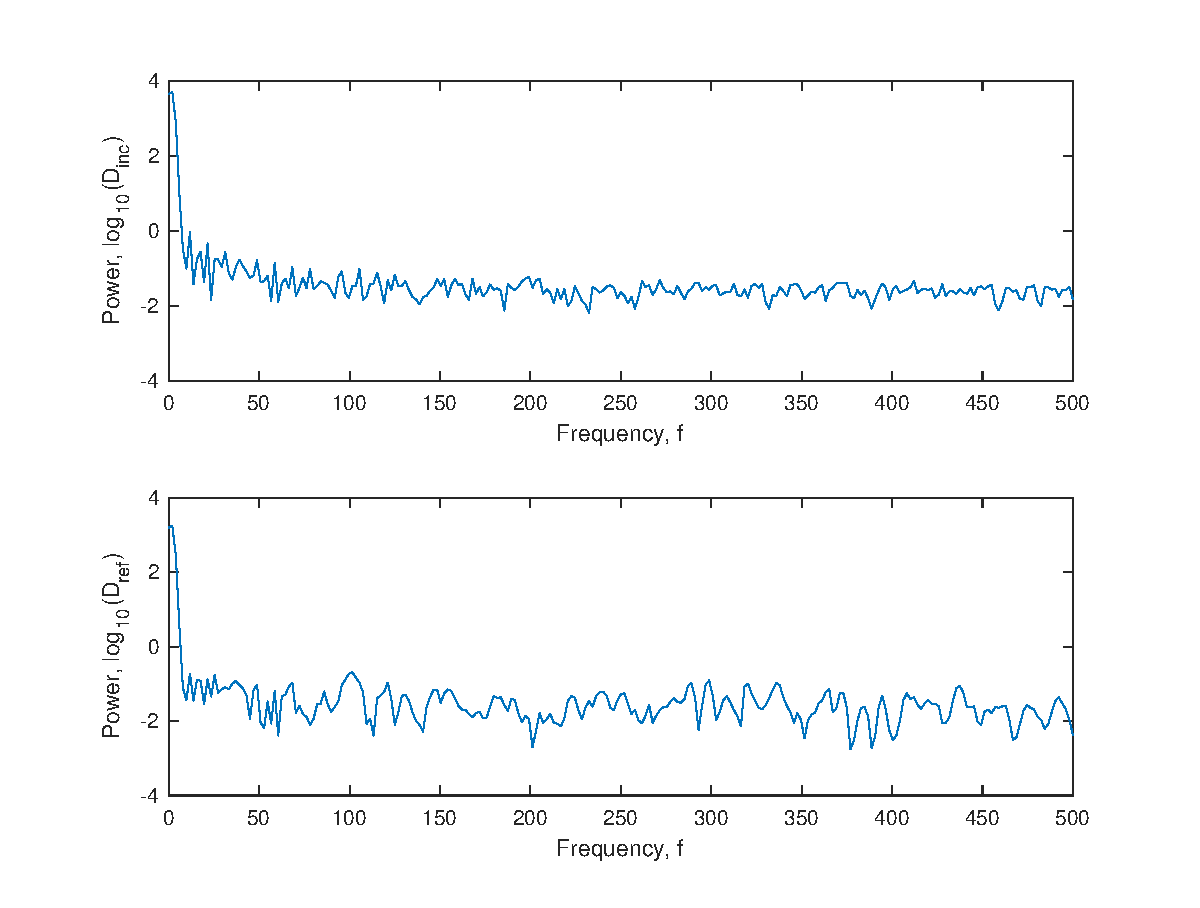
\includegraphics[width=\linewidth]{horhighres.eps}
    \caption{Power spectrum for the distance of the incident and reflected shock wave from the wall.}
    \label{fig:my_label}
\end{figure}



As we expected the power spectrum are almost identical just that the latter to contain more noise, this is due to the fact that our vertical knife edge highlights the shock wave picking up less of the behaviour going on in the periphery. The horizontal knife edge picks up more of this and hence the technique of measurement of the shock wave position is not as accurate. We still observe similar peaks in all though. \par



To evaluate the boundary layer thickness unfortunately the was to much noise to use a clear cut edge function so point were marked with a cutoff criteria as to deem the edge of the boundary later. We can calculate the turbulent boundary layer thickness pre-shock as
\begin{equation}
    \delta_{pre} = 0.0070 mm
\end{equation}
We can do exactly the same thing for the boundary layer post shock bubble and calculate here the boundary layer thickness to be 
\begin{equation}
    \delta_{post} = 0.0133 mm
\end{equation}
The observable difference is the separation region induced by the shock boundary layer interaction which lifts the boundary layer of the wall of the wind tunnel by these results the boundary layer thickness appears to double. We will refer back to these results one we have some results for the frequency and can calculate a Strouhal number with this result. \par





\vspace{5mm}
\centerline{\textbf{Vertical knife edge - high frequency}}
\vspace{5mm}





The higher sampling rate allows us to estimate the oscillating frequency of the shock wave, for both incident and reflected waves. Unfortunately the method does not extract the clearest result but the shock oscillation as indicated in Figure 9 is expected to be around $f_{inc} = 265.625$. For the reflected wave this is calculated to be slightly slower, given by $f_{ref} = 203.125$ most likely due the the interference coming from the boundary layer, the power spectrum and both these frequencies are observed in Figures 11 and 12. \par 



\begin{figure}[H]
    \centering
    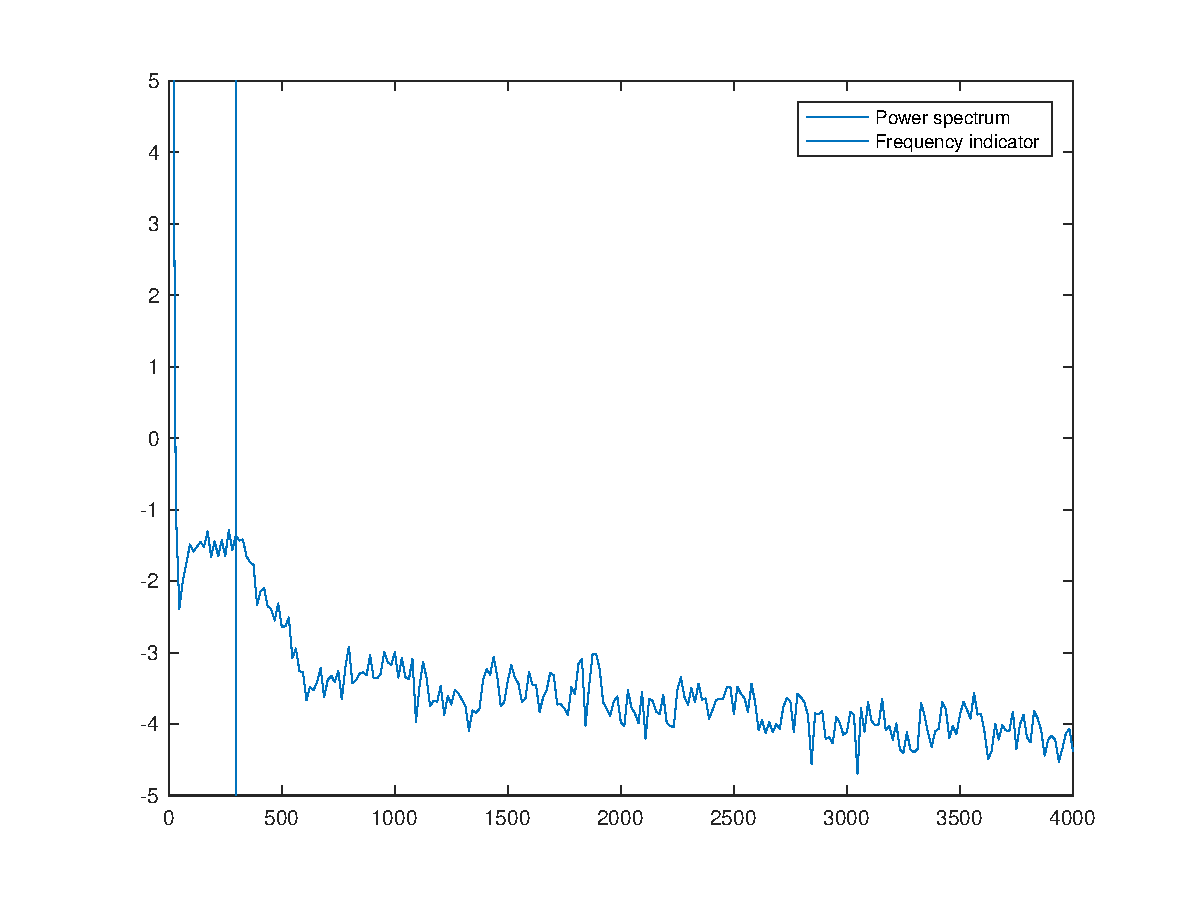
\includegraphics[width=\linewidth]{verlowresinc.eps}
    \caption{Power spectrum for the incident shock wave.}
    \label{fig:my_label}
\end{figure}



\begin{figure}[H]
    \centering
    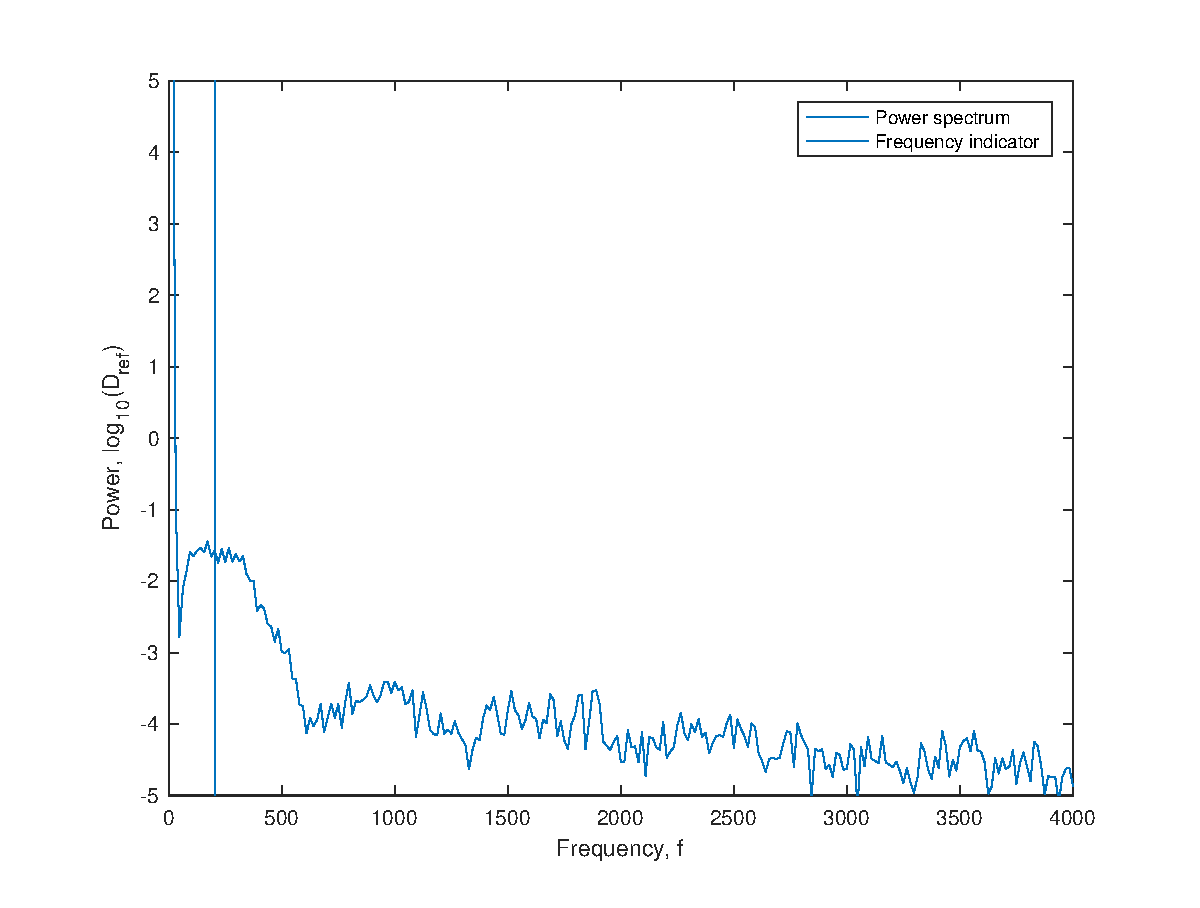
\includegraphics[width=\linewidth]{vertlowresref.eps}
    \caption{Power spectrum for the incident shock wave.}
    \label{fig:my_label}
\end{figure}



Lastly we move on to the last measurement of the oscillations of the shock bubble in which multiple methods were attempted to extract these oscillations. Various polynomial curves were fitted to regions without much luck so then the intersection of line coming for incident and reflected waves given the power spectrum seen in Figure 13. The shock bubble oscillations we would expect to be of the same order as the shock waves we calculate these oscillations in a similar way the the shock waves (please refer back to Figure 1 where the shock bubble is approximated and the highlighted yellow line is approximated by a parabola then the distance between this parabola and a reference point is measured. The power spectrum gives us peak at round $F_{bubb} =  281.25 $.



\begin{figure}[H]
    \centering
    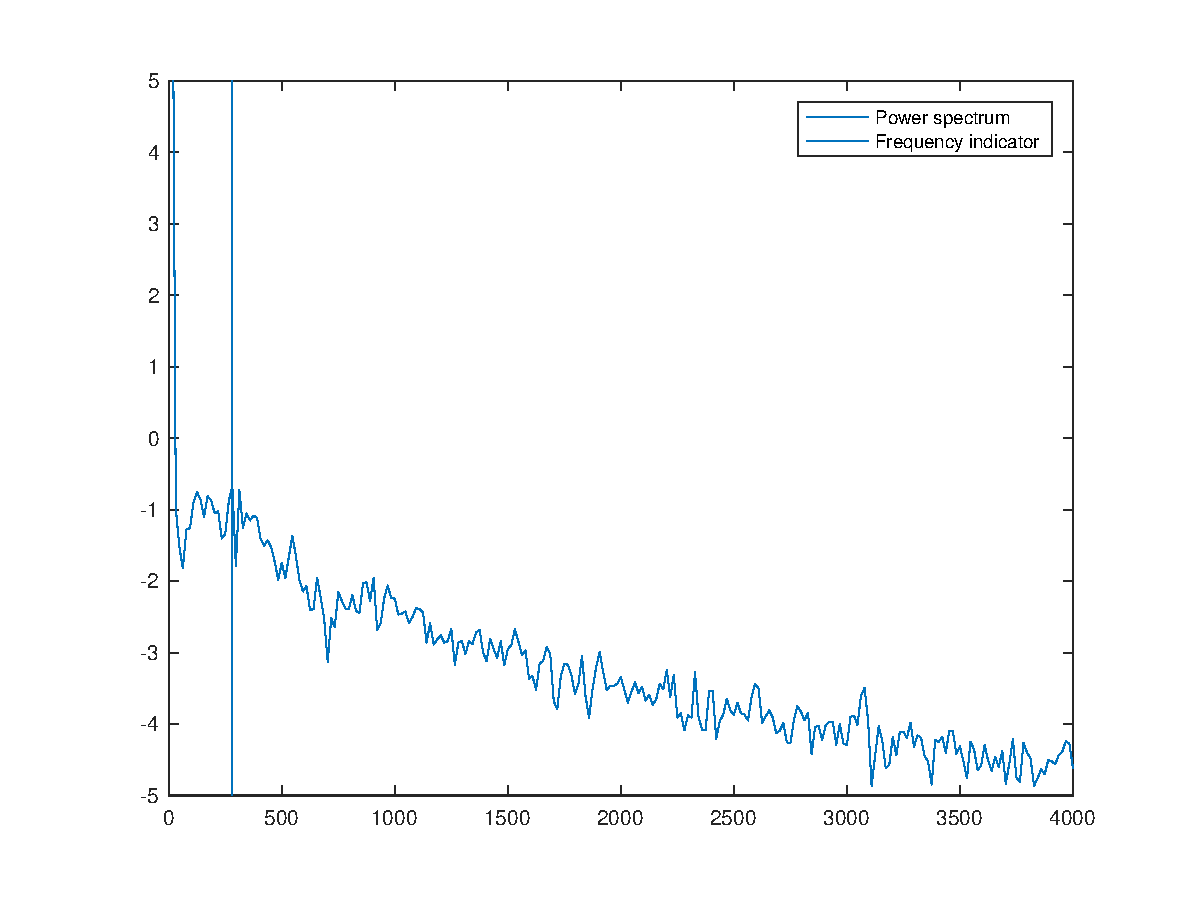
\includegraphics[width=\linewidth]{bublowres.eps}
    \caption{Power spectrum for the incident shock wave.}
    \label{fig:my_label}
\end{figure}



We can now now to the concluding topic of this section, we can calculate two Strouhal numbers for this governing flow field. The first uses the length scale of the separation bubble in which to evaluate the Strouhal number \cite{5} defined to be
\begin{equation}
    St = \frac{f L}{U_\infty},
\end{equation}
where $f$, $L$ and $U_\infty$ are the frequency, length scale and free-stream velocity. Firstly using the length scale of the separation bubble 
\begin{equation}
    St_{bubb} = 0.0160.
\end{equation}
Carrying out the same analysis with the other proposed mechanism that is waves of characteristic length 10 $\delta_{pre}$ in the turbulent boundary layer, this time we calculate
\begin{equation}
    St_{bl} = 0.0134.
\end{equation}
So in the two cases there is not a large amount of difference in the two Strouhal numbers, the larger of the two agrees slightly between with the calculations in \cite{3}, \cite{5}, \cite{6} and \cite{7}, but both lie in the range of possible Strouhal numbers





\vspace{5mm}
\centerline{\textbf{Experimental errors}}
\vspace{5mm}





The first errors to be discussed are that of the method of shadow graph or Schlierin imaging. The quality of the images analysed plays the most important role in the ability to measure all calculation given in this report. The quality of these images depends on several factors. The initial point source has a certain amount of diffusivity to it which means that the light source is hard and doesn't correlate properly. To correct this one can place an iris/mirror after the light source. This can reduce the contamination by reducing the number of diffusive rays that reach the first lens/mirror where the smaller this device the more effective the filtering is. We can then use a condenser again to reduce diffusivity and increase collimation. \par



Next we must consider the bandwidth of the light. In this experiment white light was used and this is actually not the most ideal type of light to be used in this sort of experiment. This is because the index of refraction, outline in Section I, the Gladstone dale constant depends on the wavelength. This causes a blur in the image which makes the post processing more difficult as the edge lines are more difficult to define and pick out. Because of this narrow bandwidth sources produce better quality images where an example would be a LED light or using the previously mentioned filtering of the light. \par



The method of collamination, that being mirrors or lenses each have their own drawbacks. Lenses, when the size is increased being to become impractically expensive such that mirrors are almost always used. Both obviously though can never be created perfectly and this results in aberrations, which become worse as the size of these object increase. Both surfaces can also becomes contaminated which in turn causes light to be reflected in different ways resulting again in distortion of the image. These problems can be improved obviously by better equipment and regular checking of lens cleanliness and maintenance. \par



Next the images used in the analysis of almost of this report the images used were very noisy, even after a large amount of processing the distances measured leading to power spectrum would be thrown of every once in a while. This corruption in the data made gathering any valid results hard. \par



Lastly we are not completely sure that the oscillations that we are measuring are induced by the underlying flow mechanism depending on the measurement region taken if you chose a region where locally induced turbulence appears then this would be the frequency highlighted in the power spectrum. Now an attempt was made to choose a region where this is less likely to happen but due to the vast number of images it is not possible to search through everyone as to make sure this does not occur. \par 





% ==================================================================== Summary and conclusion ===================================================================





\section{Summary and conclusion}



Firstly the technique of Schlierin imaging was introduced as well as some back round theory on shock waves and boundary layers. Due to the popularisation of this topic in the last century from the literature, in our flow configuration we expected that in our flow configuration we would have a shock wave forming on the corner which is reflected of the other wall of the wind tunnel. As we have supersonic flow there will be a turbulent boundary layer present which has a complex interaction with the shock waves present in the flow. A separation bubble is present where the shock waves induce separation of the boundary layer.  \par



We then outlined the experimental procedure and set-up taking careful consideration of the structure of the wind tunnel and features of the wedge fixed in the test section of the tunnel. A Mach number of two was configured for the experiment. \par



Three measurements using Schlierin were taken using image processing techniques. There were vertical and horizontal knife edge measurements at high resolution and low frequency. The idea being that these two techniques offer different information about the governing flow field. These measurements allowed one to calculate the angles for all the incident, reflected and Mach line, then using the first a better approximation for the Mach number could be calculated. Using this Mach number the free stream velocity and Reynolds number could also be evaluated. Using the horizontal knife edge measurements, these quantities could be calculated again but also approximations for the boundary layer thickness deemed. These data allowed for the evaluation that the reflected shock is less steady dut to being downstream of the boundary layer interaction. \par 



A lower resolution, higher frequency set of measurements were taken next allowing for calculation of the oscillations of both incident and reflected the shock bubble. Similar frequencies are identified for the incident, reflected wave and shock bubble which then allows for estimations of Strouhal number using length scale for the two possible governing mechanisms of the flow. In this similar predictions are seen but with the shock bubble mechanism given a better estimation. This with the other high resolution results seem to imply that the shock bubble mechanism induces oscillations in our system not turbulent boundary later waves. \par


Lastly some of the drawback of this experimental method were outlined the large majority due to failures of the equipment use and he inability to completely control light. Lenses are to expensive so mirrors, which are susceptible to contamination, are used but the light is not perfectly transmitted in parallel lines which means that in nearly all cases the images aren't clear which makes analysis more difficult. That being said enough can be gathered from these images to deduce a substantial amount about the given flow, nearly all features can be evaluated in this shock boundary layer interaction and the conclusion of shock bubble induced vibrations deduced. 





% ========================================================== Recommendations for future work ===================================================================





\section{Recommendations for future work}





It would be constructive to calculate the same experiment again with the power spectrum calculated with pressure calculations. This would allow for comparison with the results of this report and be a considerable amount more accurate than the method outlined above. \par

Other options for future measurements are alternative flow set-up which also produce shock boundary layer reactions. Some examples include a compression ramp or a blunt fin \cite{2}. In these flow shock bubble are also formed and cross comparison made to deem if we have and upstream mechanism forcing the system or if they agree with the shock bubble conclusion. \par





% ===================================================================== References =============================================================================





\begin{thebibliography}{9}





\bibitem{1} G.S. Settles. Schlieren and Shadowgraph Techniques: Visualizing Phenomena in Transparent Media. Springer.



\bibitem{2} J. H. Gladstone and T. P. Dale. Researches on the Refraction, Dispersion, and Sensitiveness of Liquids. Phil. Trans. R. Soc. Lond. 1863 153, 317-343.



\bibitem{3} N. T. Clements and V. Narayanaswamy. Low-frequency unsteadiness of shock wave/turbulent boundary layer interactions. Annu. Rev. Fluid Mech. 2014 46, 469-492.



\bibitem{4} Wikipedia image . https://en.wikipedia.org/wiki/Bulletbowshockwave.



\bibitem{5} P.Dupont, C. Haddad, J. P. Ardissone. J. F. Debieve. Space and time organisation of a shock wave/turbulent boundary layer interaction. Aero. Sci. Tech. 2005 561-572



\bibitem{6} P.Dupont, J-P. Dussauge, J. F. Debieve. Unteadiness in shock wave boundary layer interactions with seperation. Aero. Sci. Tech. 2006 85-91



\bibitem{7} D. Estruch, N. J. Lawson, D. G. MacManus, K. P. Garry, J. L Stollery. Measurement of shock wave unsteadiness using a high speed schlieren system and digital image processing. Rev. Sci. Inst. 2008. 79 - 126108.



\bibitem{8} F. M. White. Fluid Mechanics. McGraw-Hill.



\bibitem{9} J. K. Eaton, L. Eaton. LabTutor. Oxford University Press





\end{thebibliography}





\end{multicols}





\end{document}